\section{Bandt-Pompe Symbolization: A Background}

In our work, we consider that ordinal patterns are formed from white noise sequences using Bandt-Pompe symbolization and mapped in the two-dimensional plane of information theory descriptors, permutation entropy and statistical complexity.
Through the space formed by this tuple of features, we were able to obtain regions of confidence and a test statistic that can discriminating random series.

\subsection{The Bandt-Pompe Methodology}

Let ${\mathcal X} \equiv \{x_t\}_{t=1}^{T}$ be a real valued time series of length $T$, without ties. 
As stated by \Mycite{PermutationEntropyBandtPompe} in their seminal work:  
\begin{quote}
``If the $\{x_t\}_{t=1}^{T}$ attain infinitely many values, it is common to replace them by a symbol sequence 
$\Pi \equiv \{\pi_j\}$ with finitely many symbols, and calculate source entropy from it".
\end{quote}
Also, as stressed by these authors, 
\begin{quote}
``The corresponding symbol sequence must come 
naturally from the $\{x_t\}_{t=1}^{T}$ without former model assumptions".
\end{quote}

Let ${\mathbbm A}_{D}$ (with $D \geq 2$ and $D \in {\mathbbm Z}$) be the symmetric group of order $D!$ formed by all 
possible permutation of order $D$, and the symbol component vector 
${\bm \pi}^{(D)} = (\pi_1, \pi_2, \dots, \pi_D)$ so every element ${\bm \pi}^{(D)}$ is unique 
($\pi_j \neq \pi_k~\forall~j \neq k$). 
Consider for the time series ${\mathcal X} \equiv \{x_t\}_{t=1}^{T}$ its time delay embedding representation,
with embedding dimension $D \geq 2$ ($D \in {\mathbbm Z}$) and time delay $\tau \geq 1$ ($\tau \in {\mathbbm Z}$, also called ``embedding time''):
\begin{equation} 
\label{eq:time-delay}
{\mathbf X}^{(D,\tau)}_t ~=~( x_t,x_{t+\tau},\dots,x_{t+(D-1)\tau} ) \ ,
\end{equation} 
for $t = 1,2,\dots,N$ with $N = T-(D-1) \tau$.
Then the vector ${\mathbf X}^{(D,\tau)}_t$ can be mapped to a symbol vector ${\bm \pi}^{(D)} \in {\mathbbm A}_{D}$. 
This mapping should be defined in a way that preserves the desired relation between the elements 
$x_t  \in {\mathbf X}^{(D,\tau)}_t$, and all $t \in T$ that share this pattern (also called motif) have to mapped to the same 
${\bm \pi}^{(D)}$. 
The two most frequent ways to define the mapping ${\mathbf X}^{(D,\tau)} \mapsto {\bm \pi}^{(D)}$ are:  
\begin{enumerate}[label=\alph*)]
\item ordering the ranks of the $x_t \in {\mathbf X}^{(D,\tau)}$ in chronological order 
       (\textit{Rank Permutation}) or,
\item ordering the time indexes according to the ranks of $x_t \in {\mathbf X}^{(D,\tau)}$  
       (\textit{Chronological Index Permutation});
\end{enumerate}
       see details in \Mycite{BPRepeatedValuesChaos}.
Without loss of generality, in the following we will only use the latter.

Consider, for instance, the time series $\mathcal X = (1.8, 1.2, 3.2, 4.8, 4.2, 4.5, 2.3, 3.7, 1.2, .5)$ depicted in Fig.~\ref{Fig:IntroBP}.
Assume we are using patterns of length $D=5$ with unitary time lag $\tau=1$.
The code associated to $\mathbf X_{3}^{(5,1)}=(x_3,\dots,x_7)=(3.2, 4.8, 4.2, 4.5, 2.3)$, shown in black, is formed by the indexes in $\bm\pi^{(5)}=(1,2,3,4,5)$ which sort the elements of $\mathbf X_{3}^{(5,1)}$ in increasing order: $51342$.
With this, $\widetilde{\pi}^{(5)} = 51342$, and we increase the counting related to this motif in the histogram of all possible patterns of size $D=5$.

The dash-dot line in Fig.~\ref{Fig:IntroBP} illustrates $\mathbf X_{1}^{(5,2)}$, i.e. the sequence of length $D=5$ starting at $x_1$ with lag $\tau=2$.
In this case, $\mathbf X_{1}^{(5,2)}= (1.8, 3.2, 4.2, 2.3, 1.2)$, and the corresponding motif is $\widetilde{\pi}^{(5)}=51423$.

\begin{figure}[hbt]
\centering
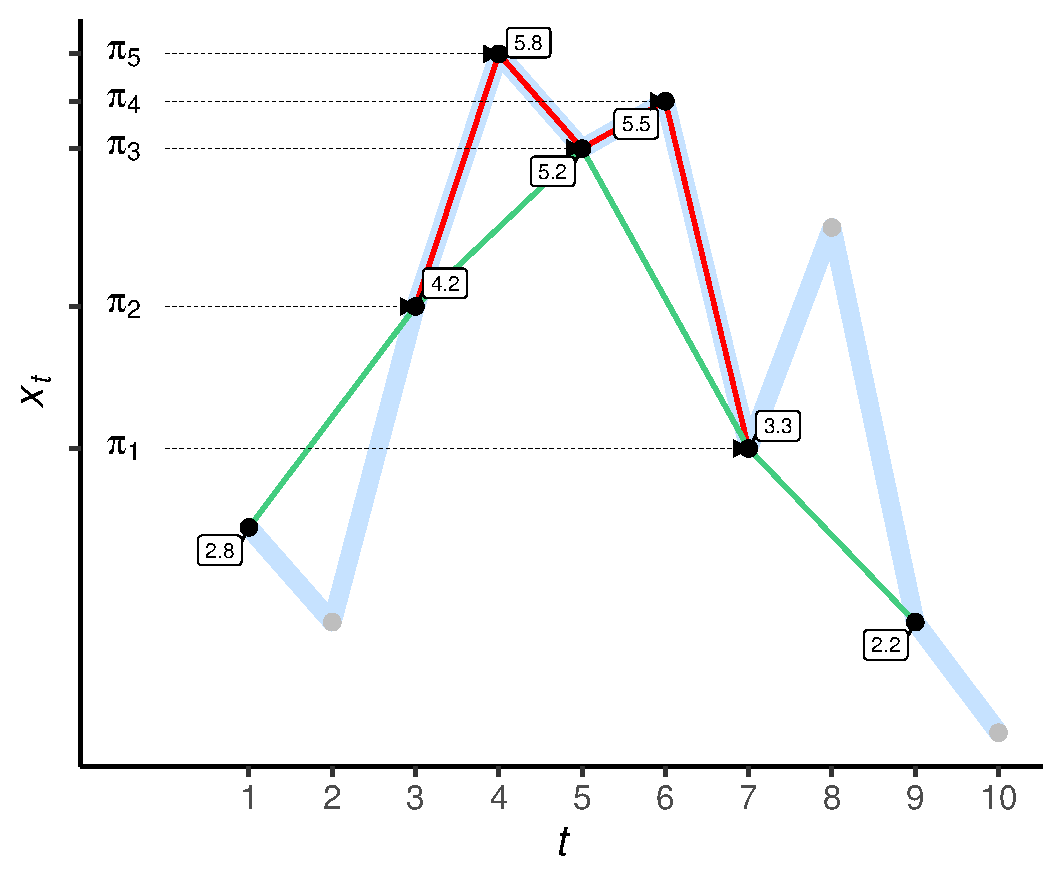
\includegraphics[width=.7\linewidth]{IntroBP}
\caption{Illustration of the Bandt and Pompe coding}
\label{Fig:IntroBP}
\end{figure}

Once all symbols have been computed, one obtains the histogram of proportions $\bm h = (h(j))_{1\leq j\leq D!}$.
This is an estimate of the (unknown, in general) probability distribution function of these patterns.
The next step into the characterization of the time series is computing descriptors from this histogram.

The first descriptor is a measure of the disorder of the system.
The most frequently used feature for this is the Normalized Shannon entropy, defined as
\begin{equation}
H(\bm h) = -\frac{1}{\log D!} \sum_{j=1}^{D!} h(j) \log h(j),
\end{equation}
with the convention that terms in the summation for which $h(j)=0$ are null.
This quantity is bounded in the unit interval, and is zero when $h(j)=1$ for some $j$ (and, thus, all other bins are zero), and one when $h(j)=1/D!$ for every $j$ (the uniform probability distribution function).

Although very expressive, the Normalized Shannon Entropy is not able to describe all possible underlying dynamics.
In particular, for intermediate values of $H$, there is a wide variety of situations worth characterizing.
To this aim, \Mycite{LopezRuiz1995} proposed using $Q$, the disequilibrium, a measure of how far $\bm h$ is from an equilibrium or noninformative distribution.
They employed the Euclidean distance between $\bm h$ and the uniform probability distribution function.

With this, they proposed $C=HQ$ as a measure of the Statistical Complexity of the underlying dynamics.
A time series can then be mapped into a point in the $H\times C$ plane.

\subsection{The Entropy-Complexity Plane}

\textcolor{red}{Describe the boundaries}

We illustrate the use of the Entropy-Complexity ($H\times C$) with the following time series:
\begin{itemize}
\item Colored $k$-noise: white ($k=0$), $k=-1/2$, pink ($k=1$), $k=3/2$, red ($k=2$), $=5/2$, and $k=3$;
\item Chaotic logistic series $x_t = r x_{t-1} (1 - x_{t-1})$, with $r=3.6$ and $4$;
\item Deterministic series: monotonic increasing ($\log(x_t+0.1)$, $x_t=\{1,2,\dots,10^4$) and periodic ($\sin(2x_t)\cos(2x_t)$, with $0\leq x_t\leq 2\pi$ over ten thousand equally spaced points).
\end{itemize}
In all cases, we used $D=6$ and $\tau=1$.
Fig.~\ref{fig:Histograms} shows nine of the histograms produced by these series using the Mersenne-Twister pseudorandom number generator;
we omitted those corresponding to the deterministic series, as they produce one and two nonzero bins.

\begin{figure}[hbt]
    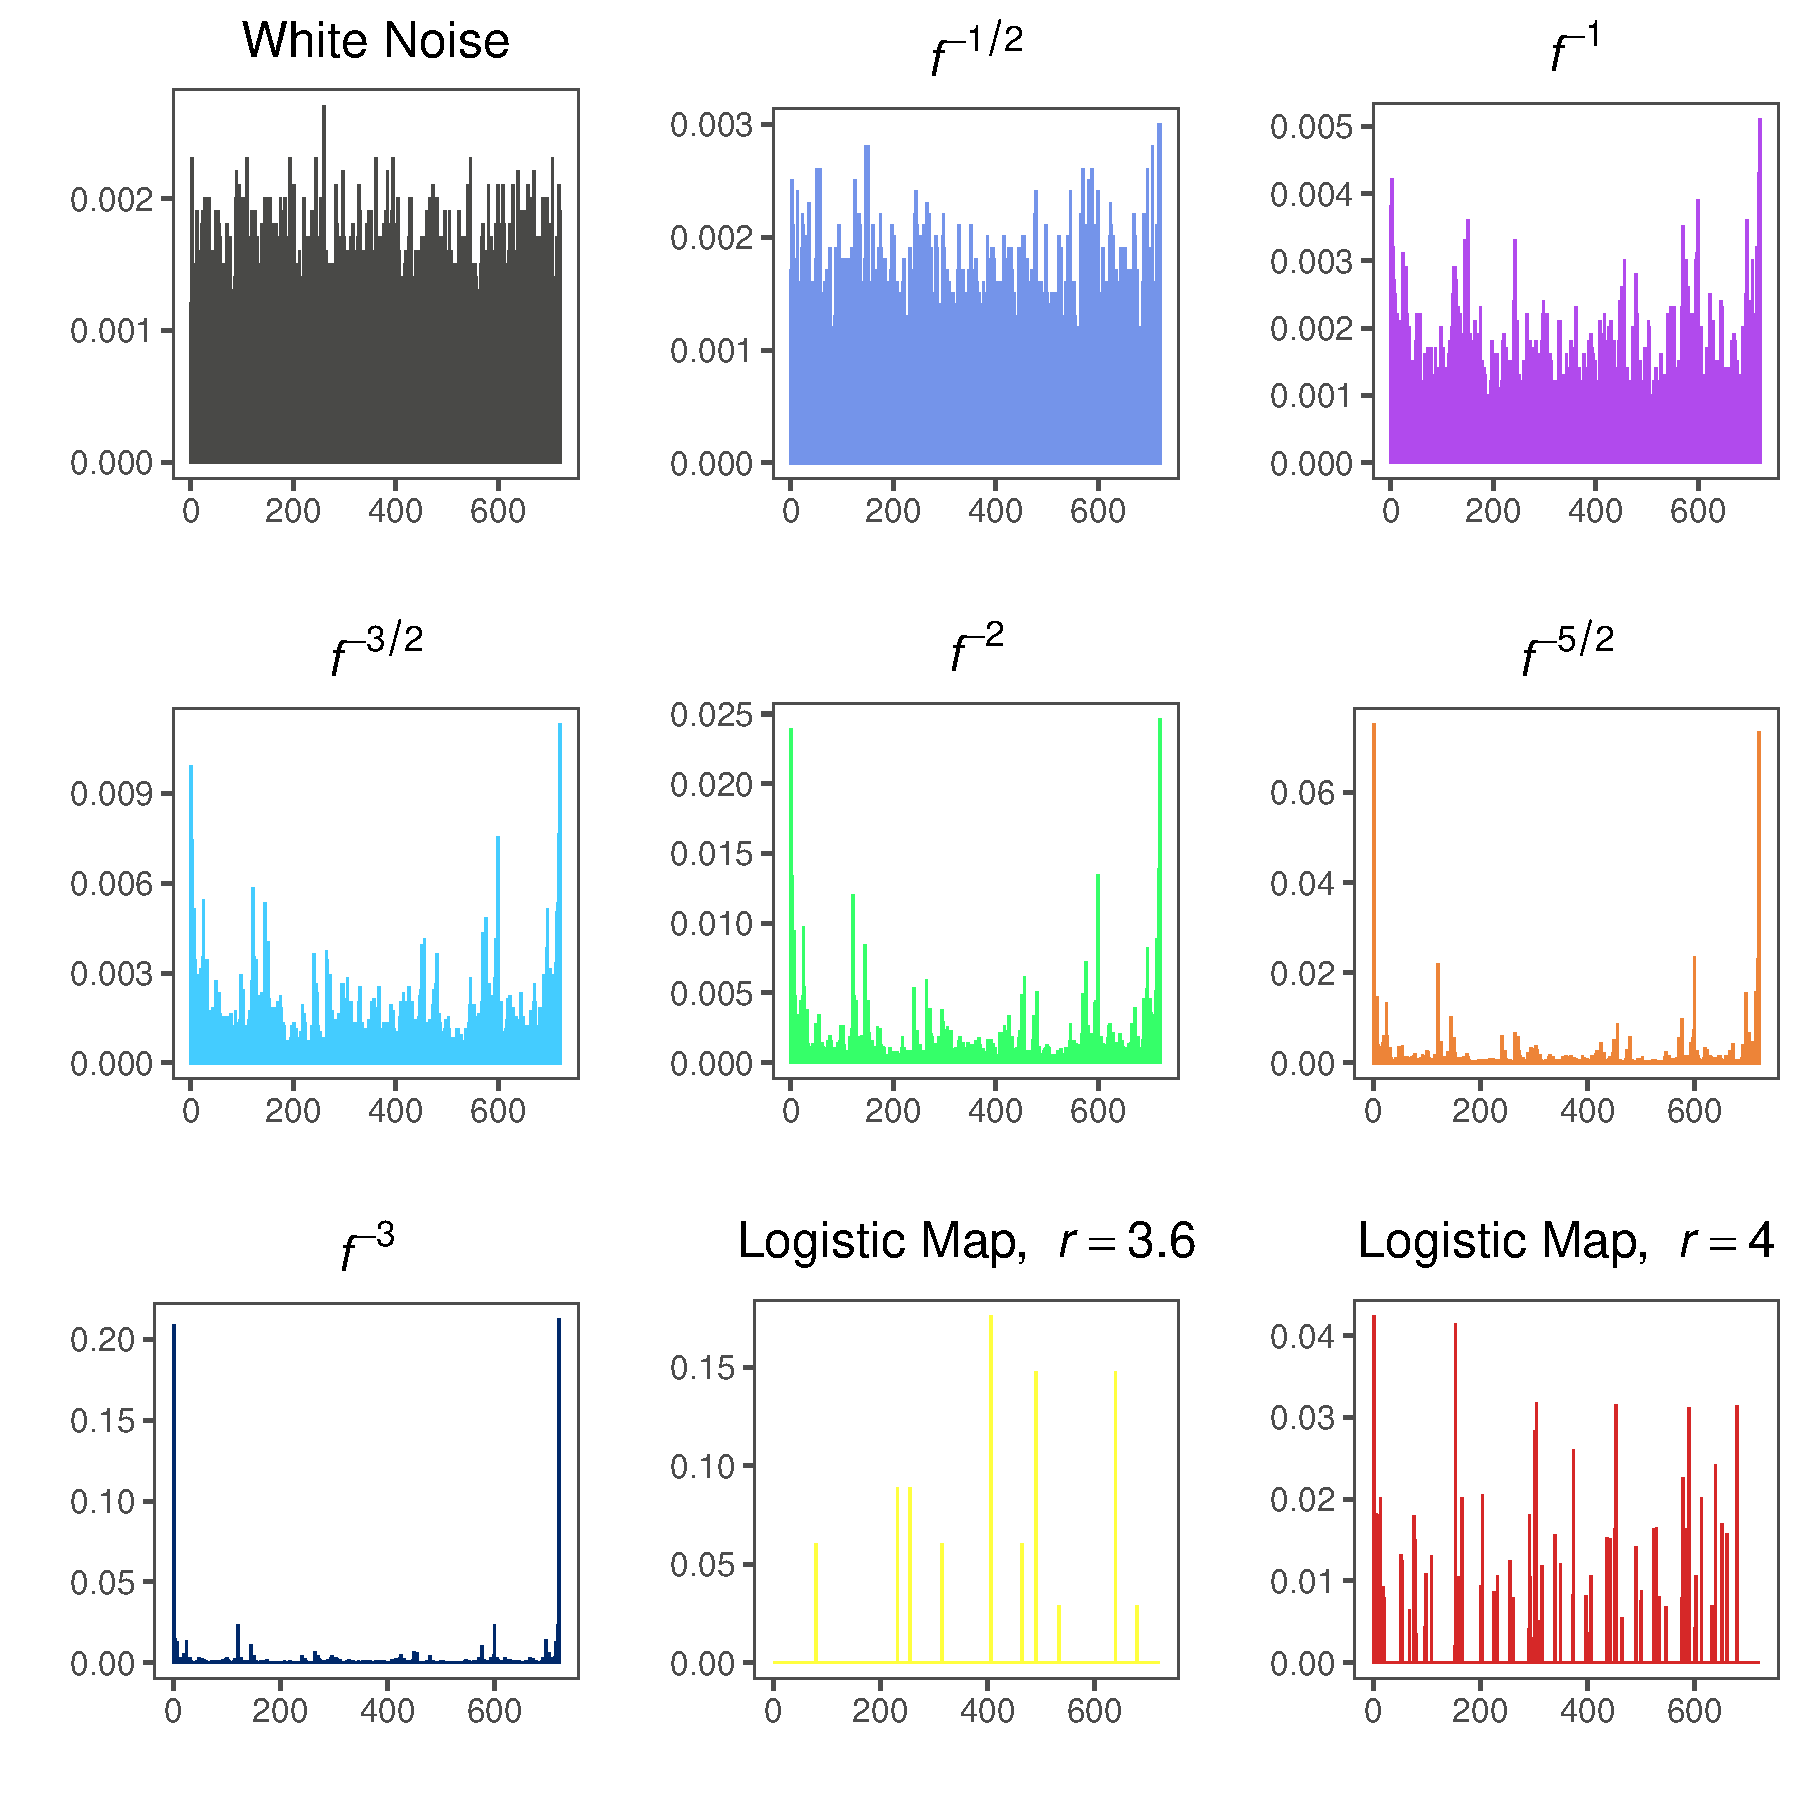
\includegraphics[width=\linewidth]{Figures/h.pdf}
	\caption{Patterns histograms of selected time series, with $D=6$ and $\tau=1$}
	\label{fig:Histograms}
\end{figure}

\begin{comment}
\begin{figure}[hbt]
\centering
	\subfloat[Logistic map $r=3.6$]{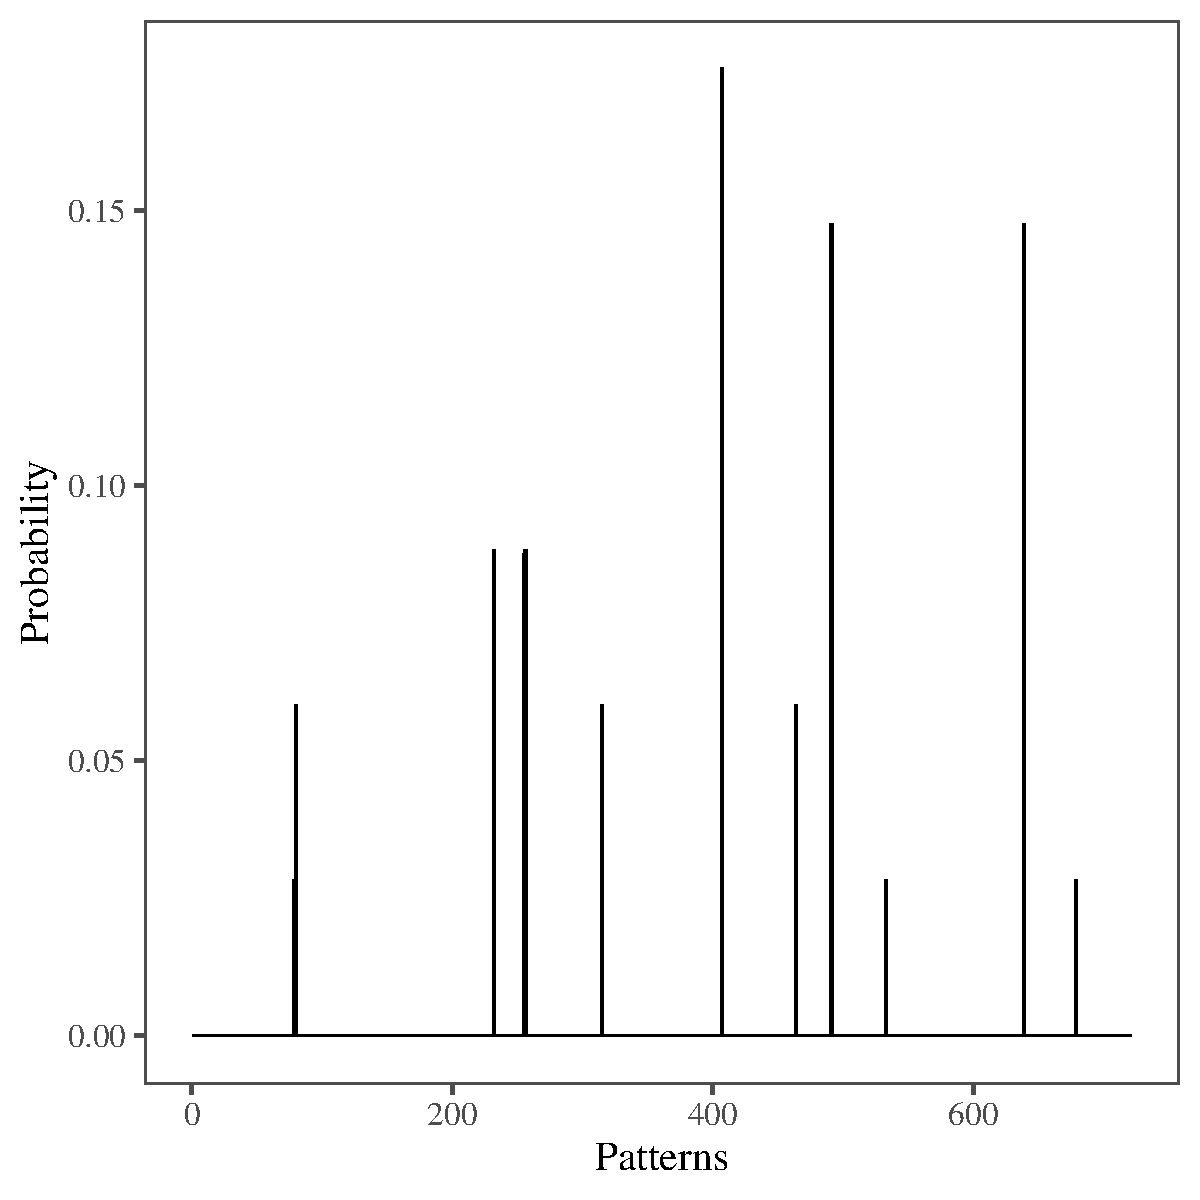
\includegraphics[width=.3\linewidth]{h36}}\quad
	\subfloat[Logistic map $r=4$]{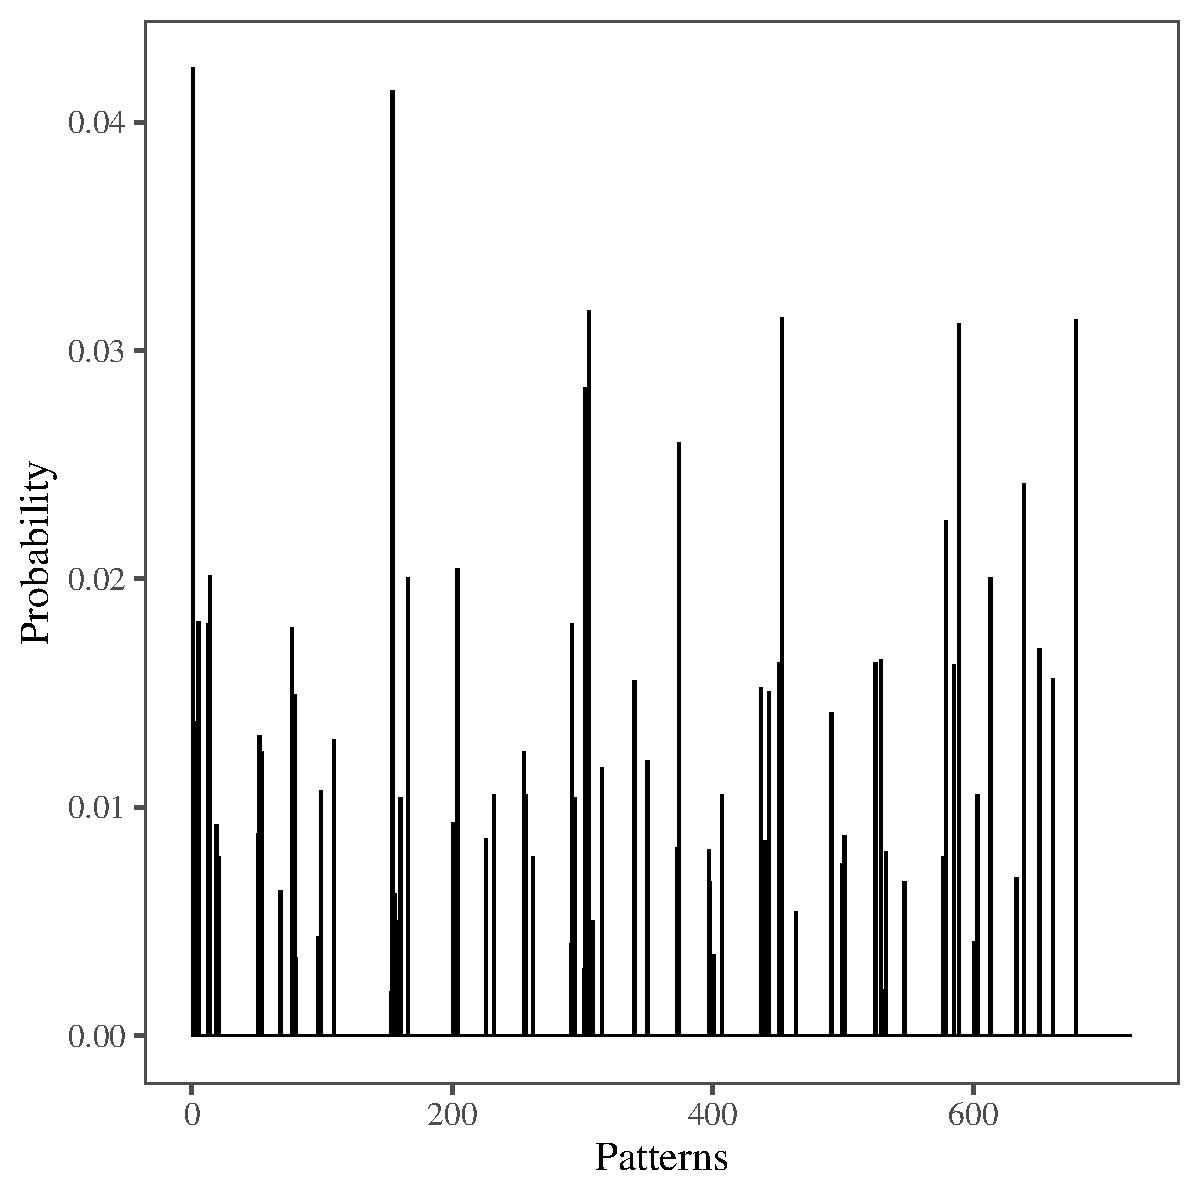
\includegraphics[width=.3\linewidth]{h4}}\quad
	\subfloat[$f^{-3}$ noise]{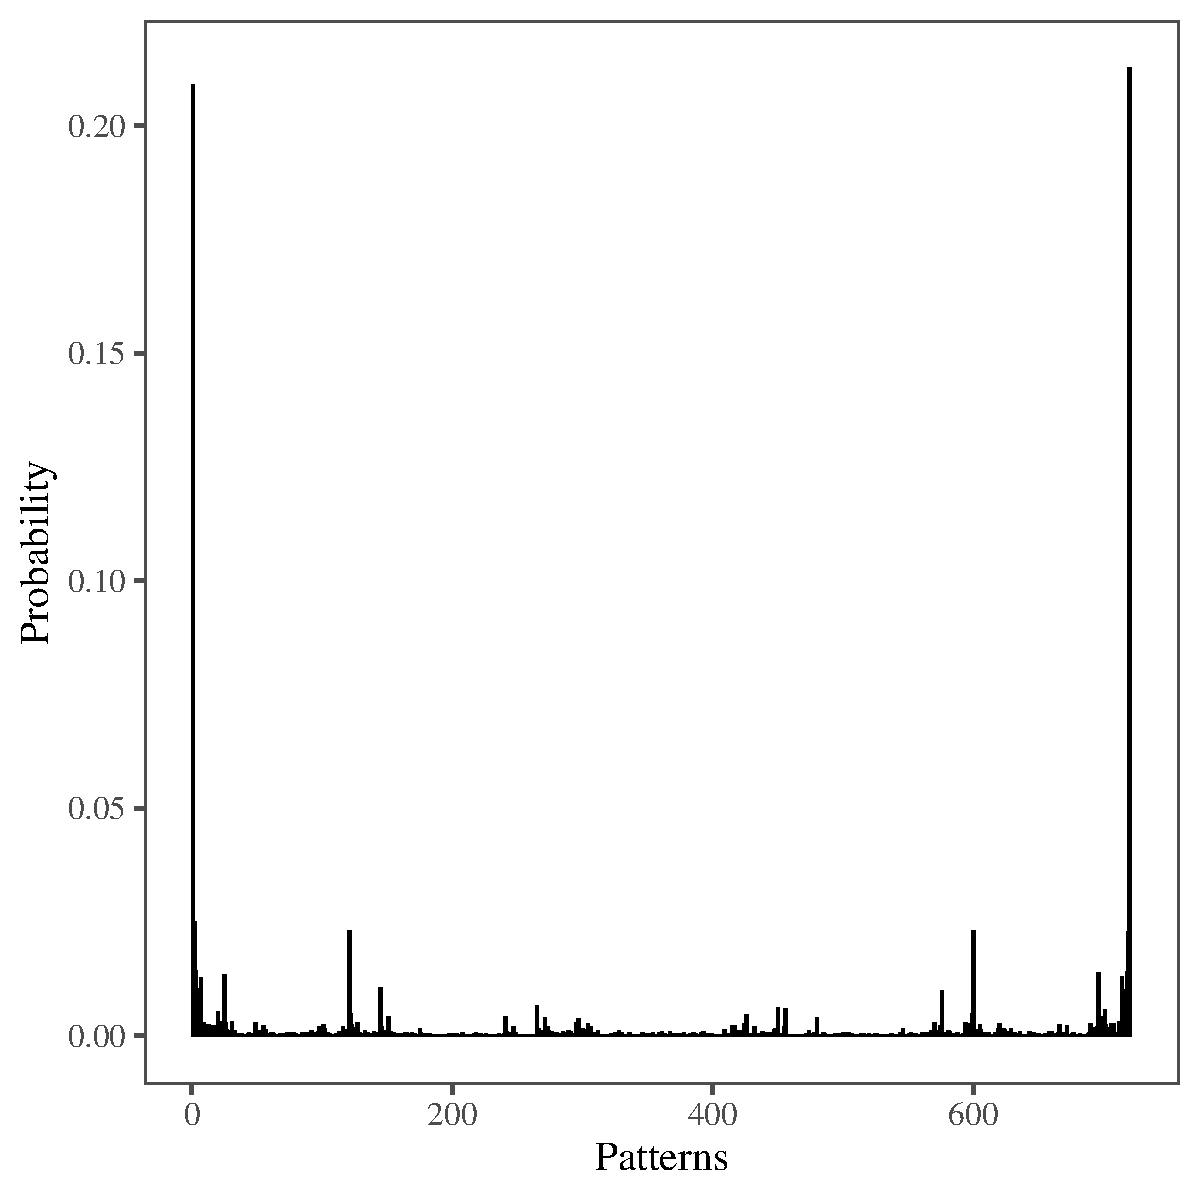
\includegraphics[width=.3\linewidth]{h3}}\quad
	\subfloat[$f^{-5/2}$ noise]{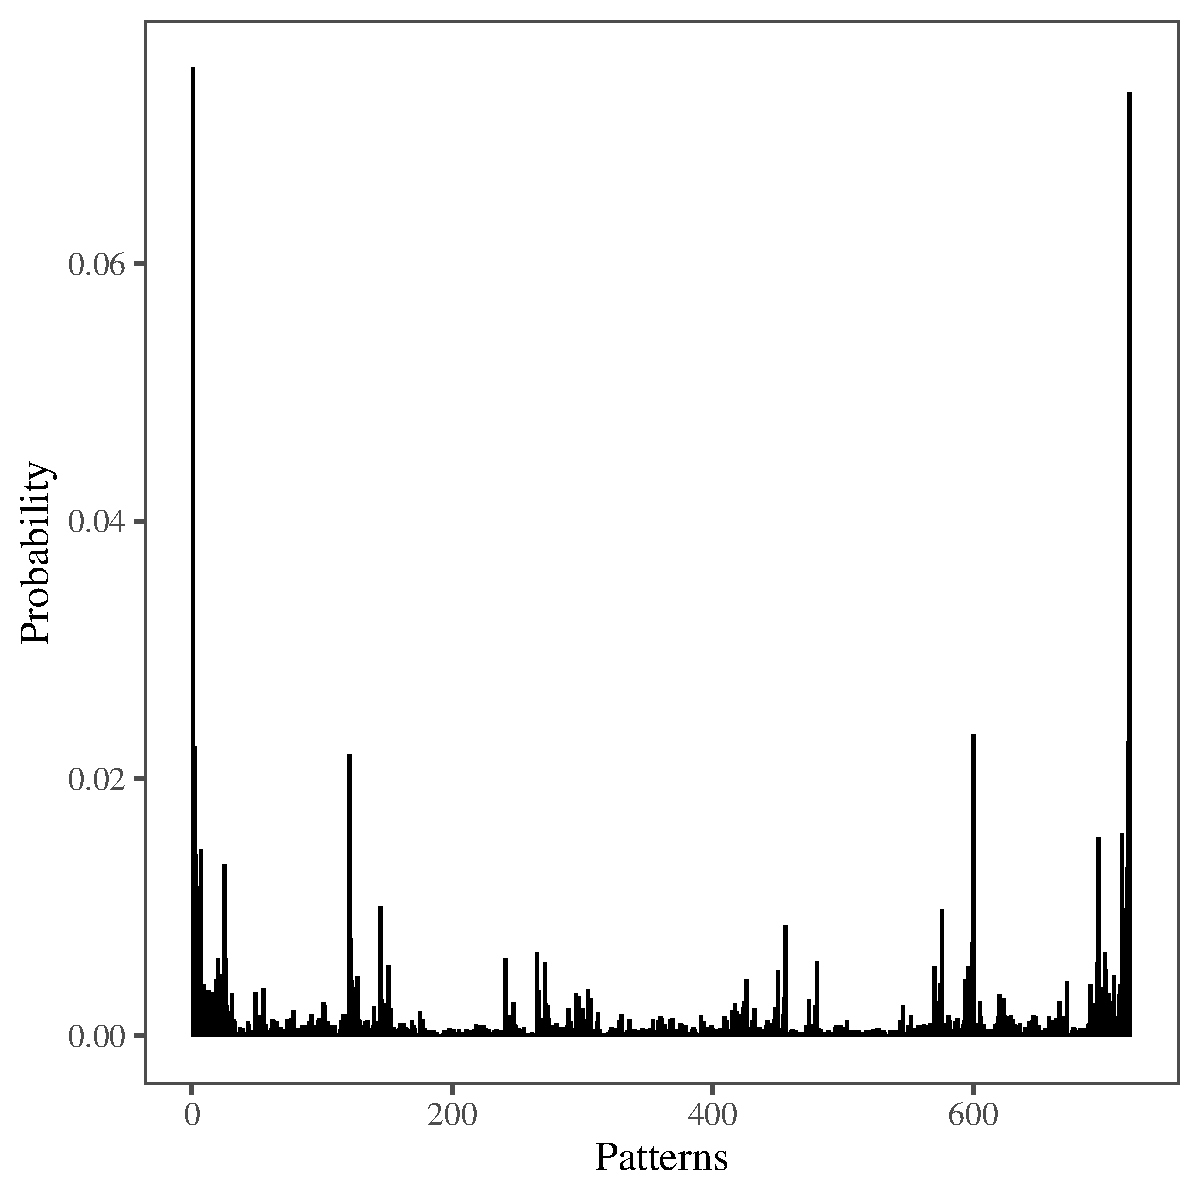
\includegraphics[width=.3\linewidth]{h25}}\quad
	\subfloat[$f^{-2}$ noise]{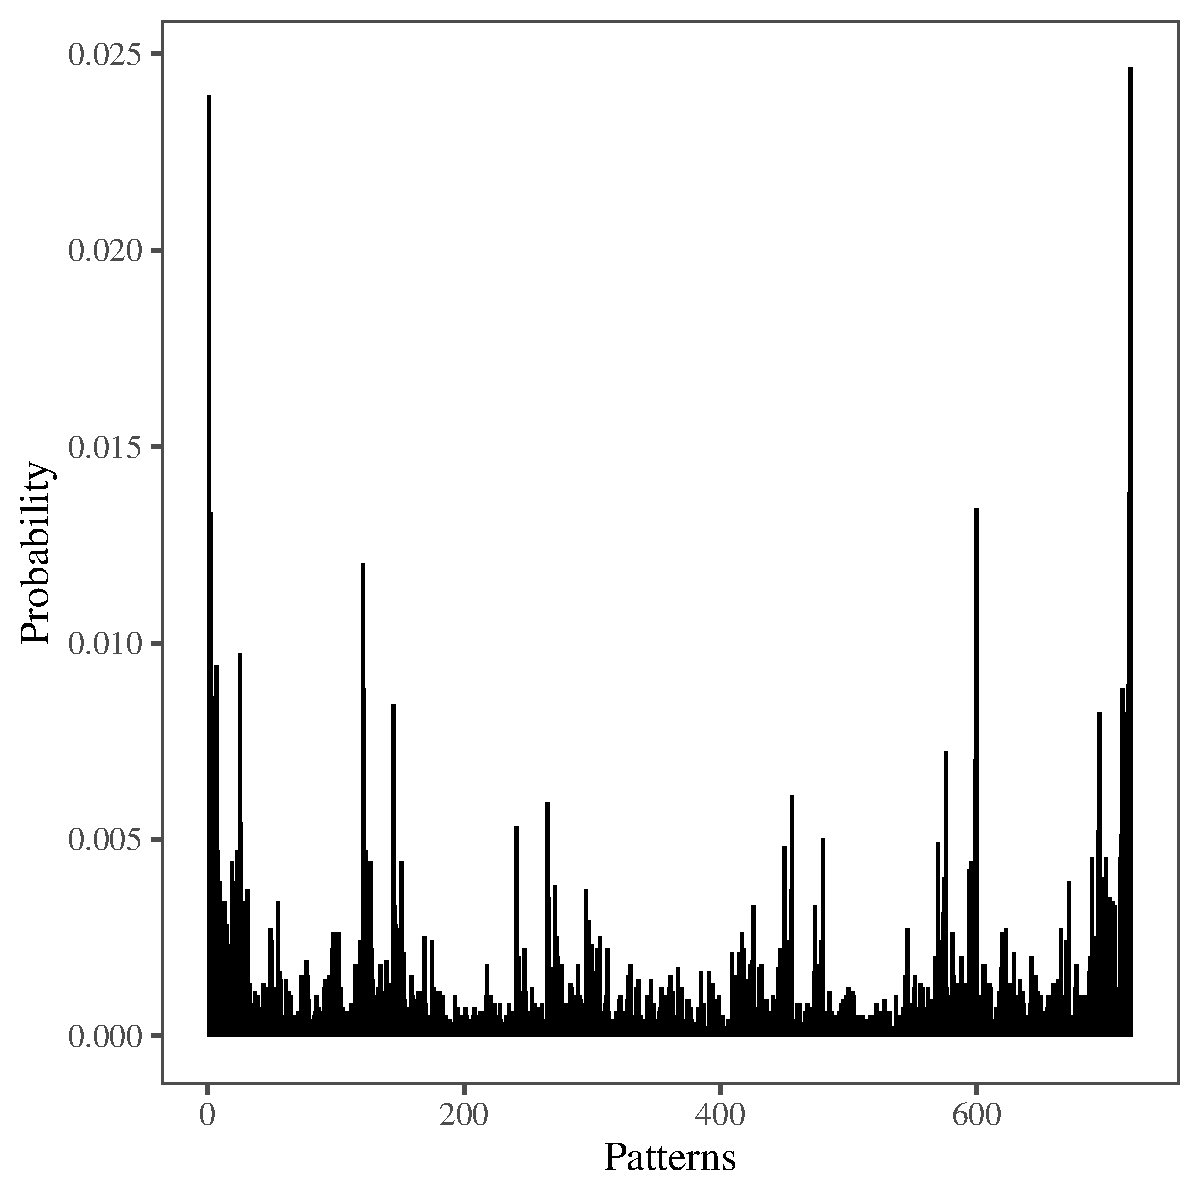
\includegraphics[width=.3\linewidth]{h2}}\quad
	\subfloat[$f^{-1.5}$ noise]{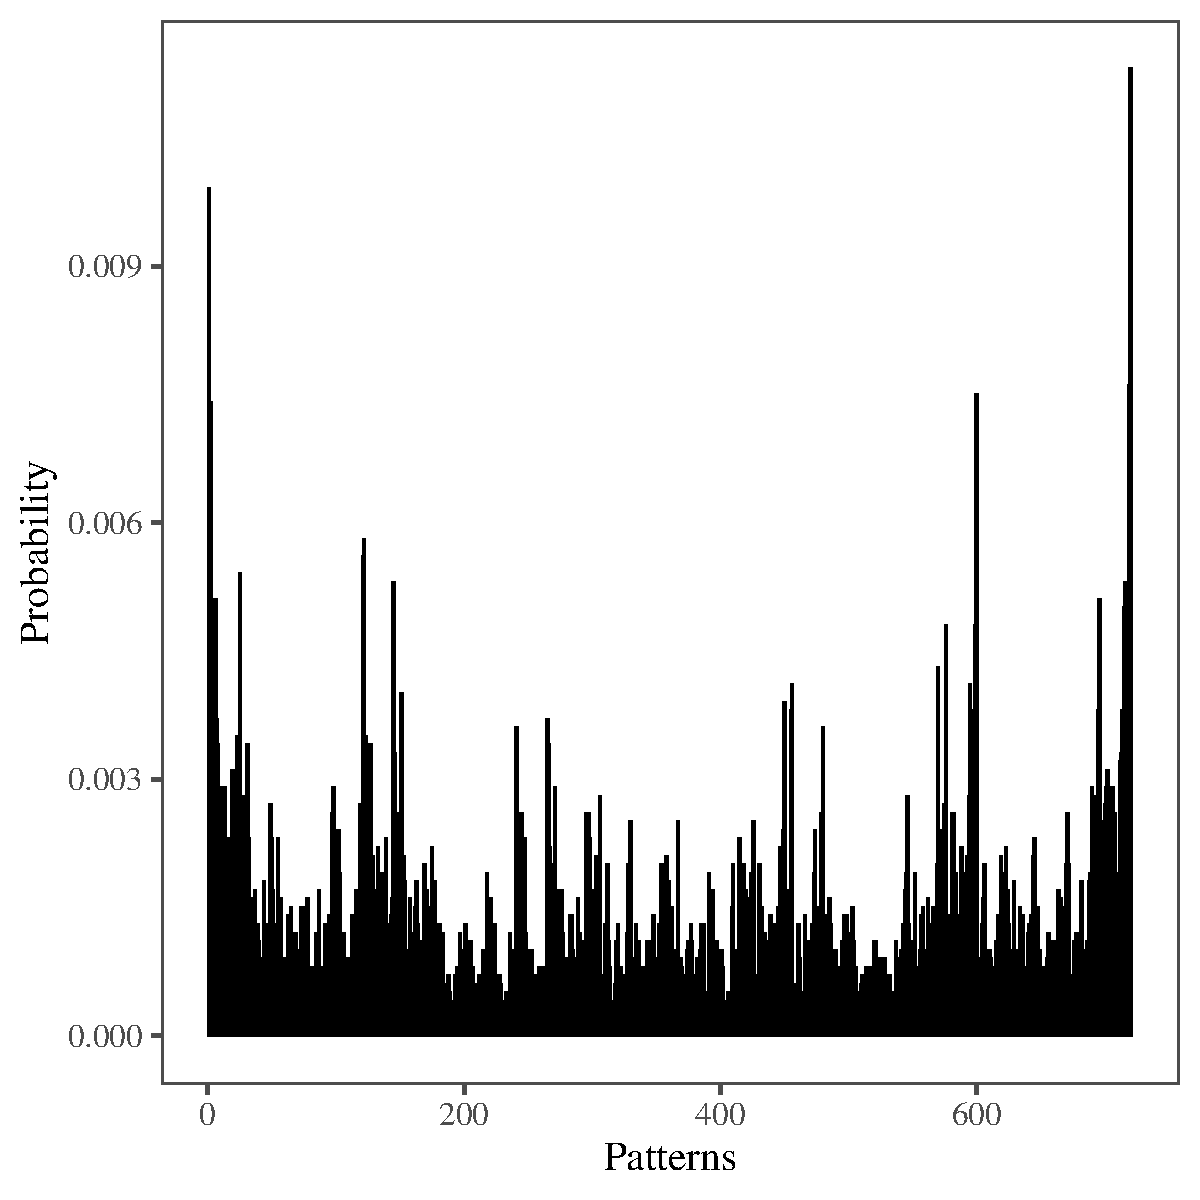
\includegraphics[width=.3\linewidth]{h15}}\quad
	\subfloat[$f^{-1}$ noise]{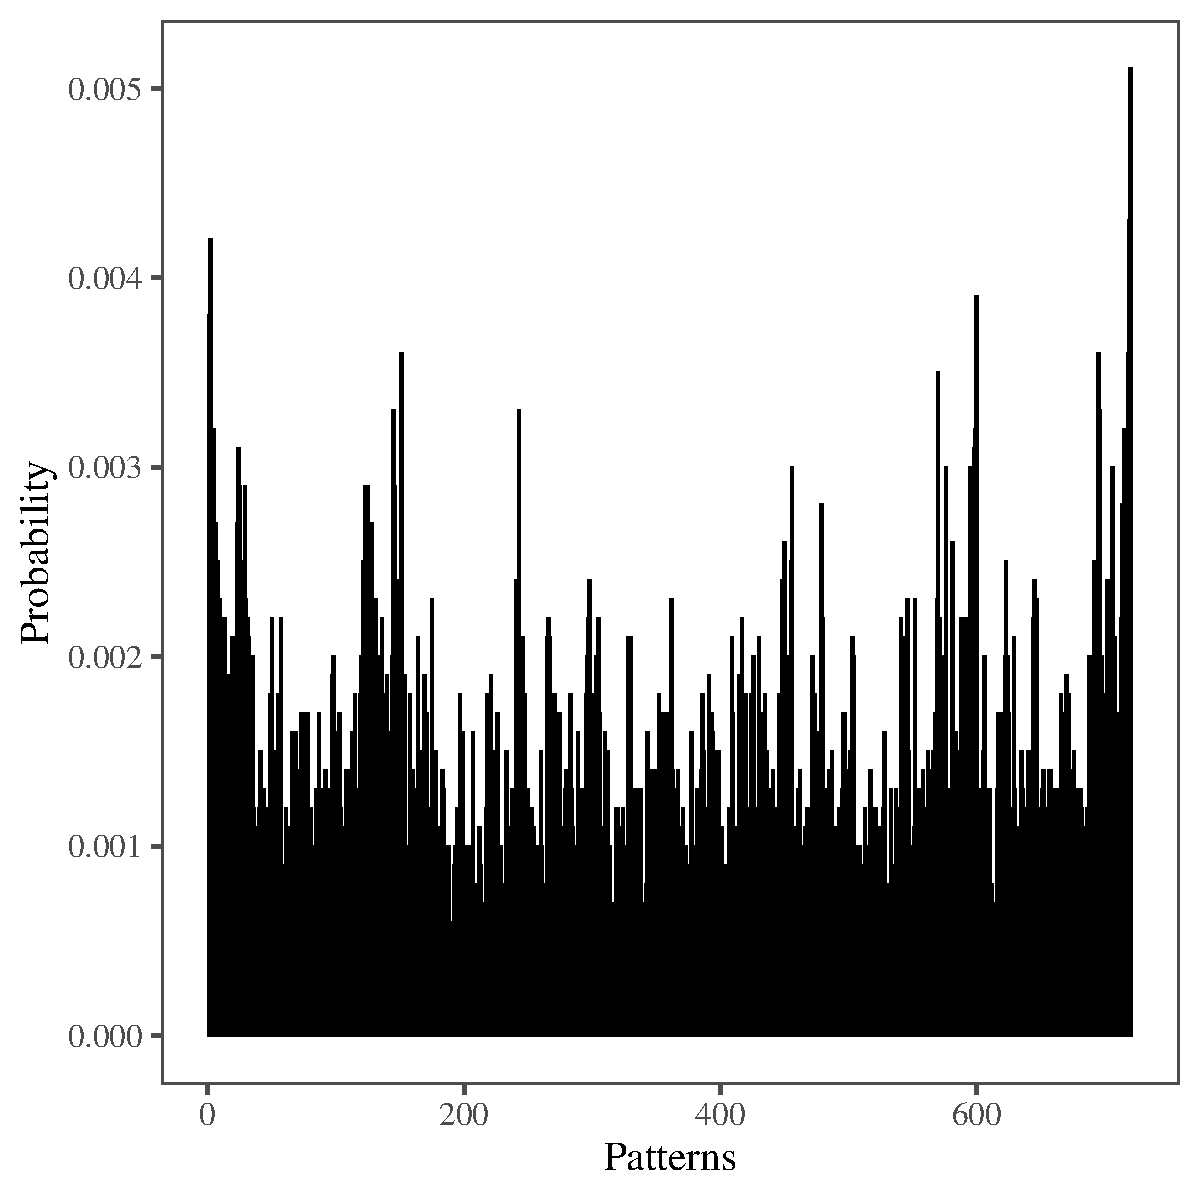
\includegraphics[width=.3\linewidth]{h1}}\quad
	\subfloat[$f^{-1/2}$ noise]{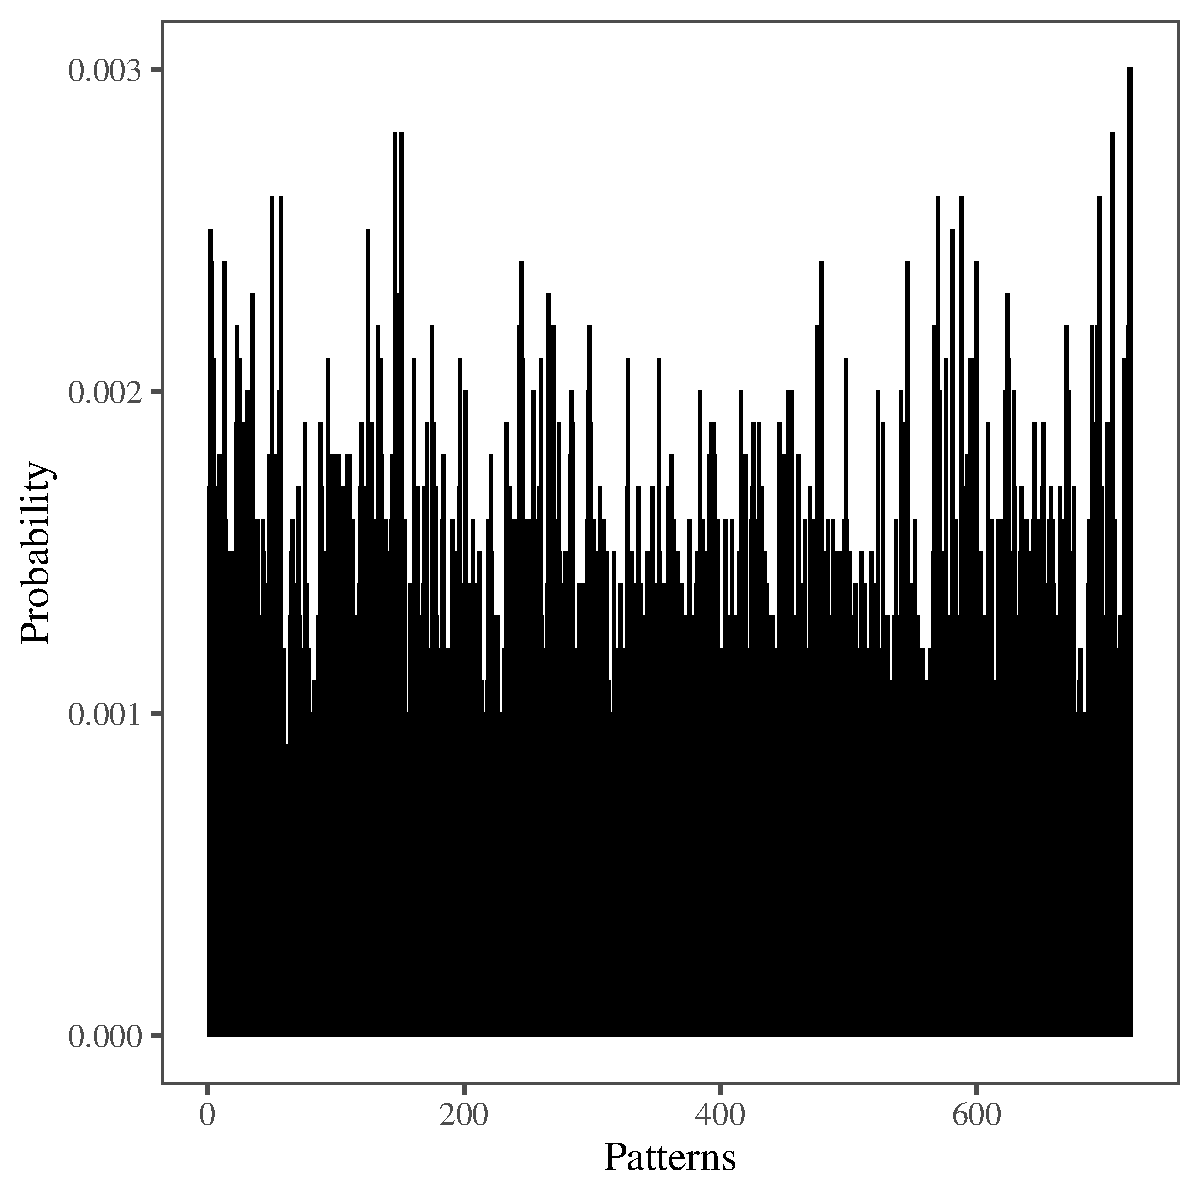
\includegraphics[width=.3\linewidth]{h05}}\quad
	\subfloat[White noise]{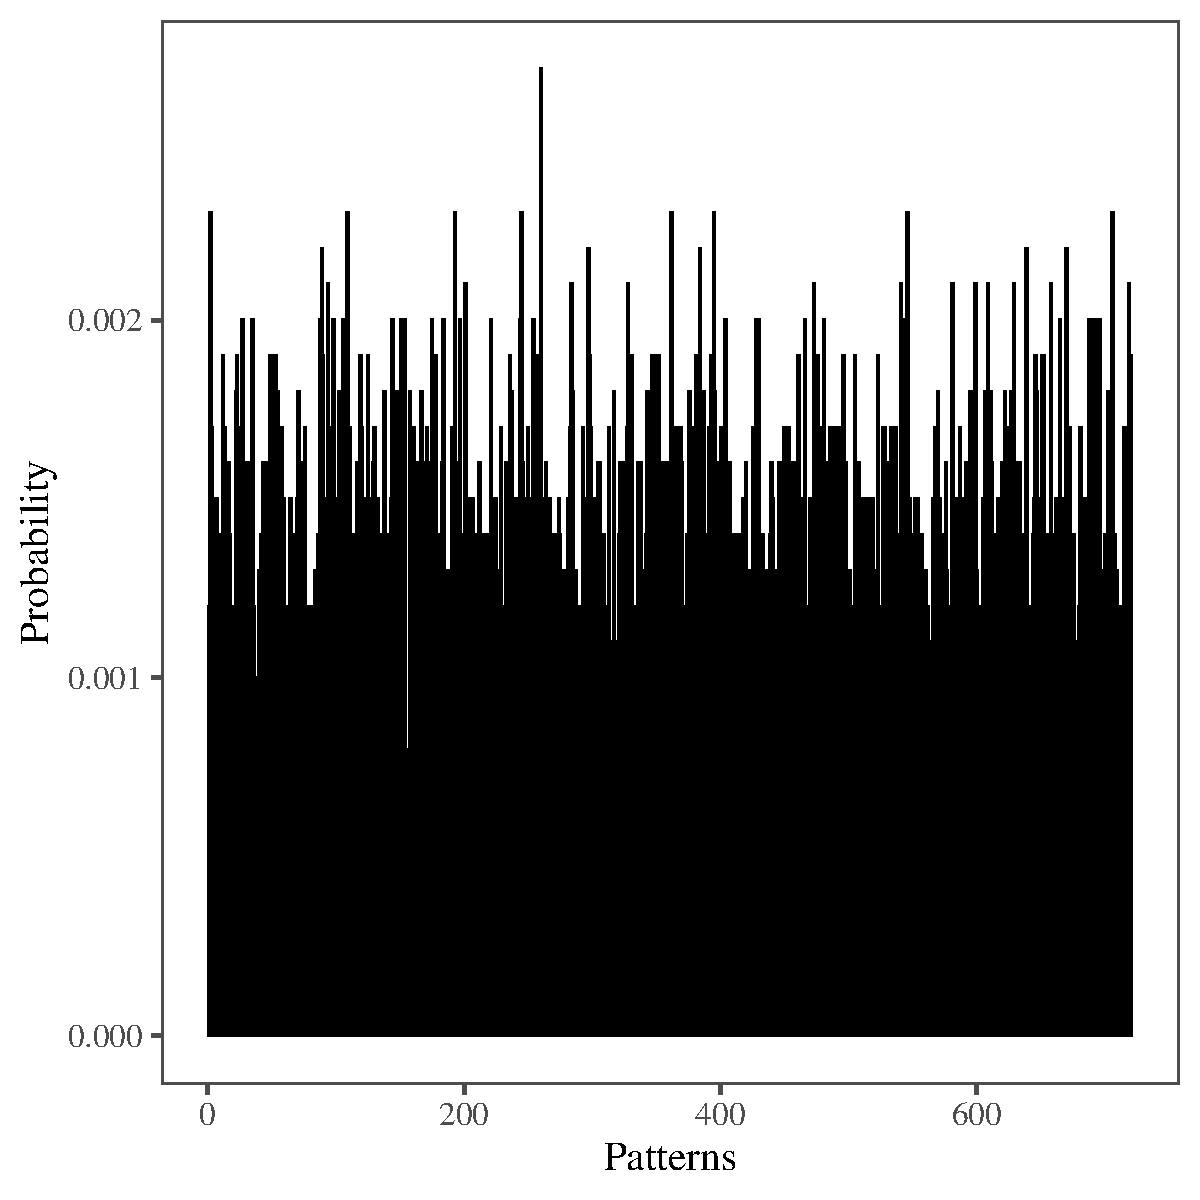
\includegraphics[width=.3\linewidth]{h0}}
	\caption{Patterns histograms of selected time series, with $D=6$ and $\tau=1$\label{fig:Histograms}}
\end{figure}
\end{comment}

Fig.~\ref{fig:AllSystems} shows the $H\times C$ plane with the bounds for $D=6$, the time series and the points they were mapped onto.
The points due to $f^{-k}$ noises appear joined by dotted segments.
It is noticeable that deterministic patterns have more complexity than random ones.
Also, points related to $f^{-k}$ noises tend to clutter for $k<1$, having the highest entropy values, as can be seen in Fig.~\ref{fig:RightMostCorner}.

\begin{figure}[hbt]
\centering
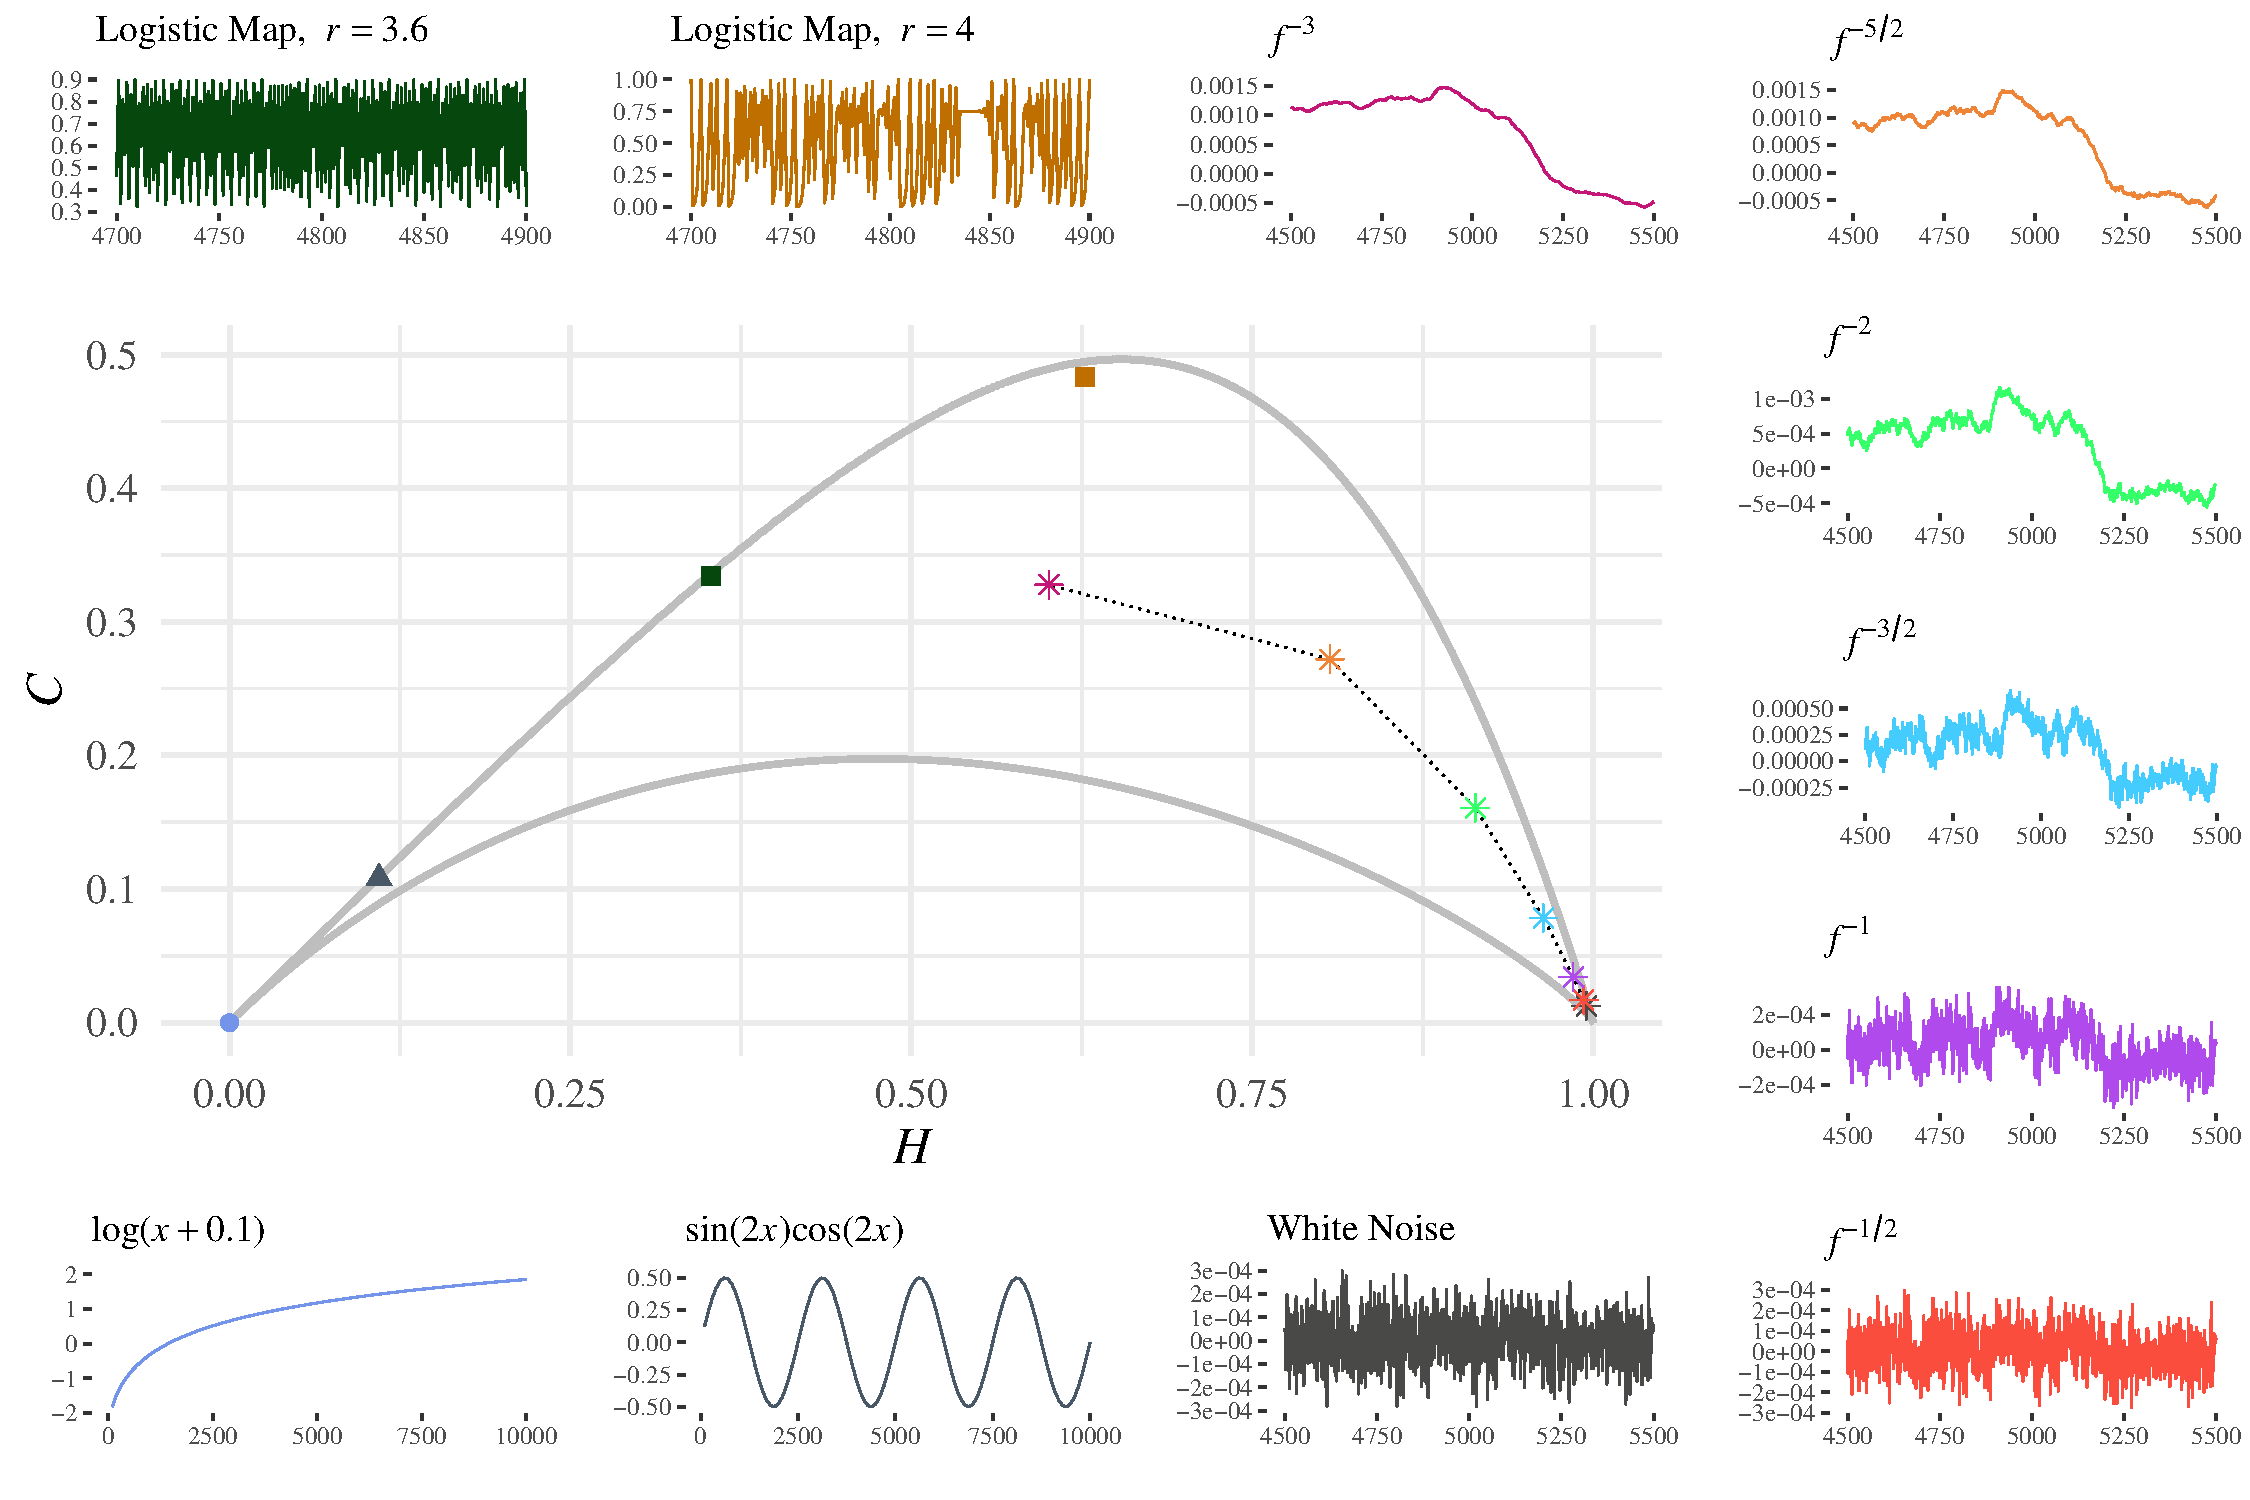
\includegraphics[width=\linewidth]{AllSystems}
\caption{Eleven systems and their points in the $H\times C$ plane}\label{fig:AllSystems}
\end{figure}

Fig.~\ref{fig:RightMostCorner} shows the rightmost lower corner of the $H\times C$ plane, emphasizing the location of the white ($k=0$), $k=-1/2$, and pink ($k=1$) noises.

\begin{figure}[hbt]
\centering
\includegraphics[width=\linewidth]{RightMostCorner}
\caption{White Noise, $f^{-1/2}$ and $f^{-1}$ noise points}\label{fig:RightMostCorner}
\end{figure}

The focus of our study is to assess pure randomness by analyzing the empirical distribution of the points produced by true random sequences, providing regions of confidence in the $H \times C$ plane.

\section{Entropy-Complexity plane in the literature}

The first works on the characterization of white noises with permutation entropy arose from the need to discriminate them in relation to chaotic maps~\cite{rosso2013characterization, xiong2020complexity, olivares2012contrasting}.
However, it was found that the measure of statistical complexity was able to efficiently quantify the performance of pseudorandom number generators, expanding the possibilities of using information theory descriptors with the Bandt-Pompe symbolization~\cite{larrondo2002statistical, gonzalez2005statistical}.

Table~\ref{Tab:Literature} presents a summary of the main works in the literature that perform analysis of non-chaotic algorithmic generators, according to their features $(h, c)$.
For this, we also provide the length $T$ and embedding dimension $D$ applied in the analysis of the time series.
The following algorithmic generators were analyzed:
\begin{itemize}
    %\item[$-$] RNG available in Intel fortran compiler (FOR)
    %\item[$-$] RNG available in Borland C++ compiler (CCC)
    %\item[$-$] Matlab RAND function (MAT)
    \item Mother RNG, available in Marsaglia website~\cite{marsaglia1994yet} (MOT);
    \item Multiple with carry RNG (MWC)~\cite{marsaglia1994yet};
    \item Combo RNG (COM)~\cite{marsaglia1994yet};
    \item Lehmer RNG (LEH)~\cite{payne1969coding};
    \item Fractional Gaussian noise with $\alpha = 0$ (fGn);
    \item Fractional Brownian motion with $\alpha = 1.2$ (fBm);
    \item $f^{-k}$ noise with $k = 0$;
    \item Linear Congruential Generator (LCG)~\cite{knuth1997sorting}.
\end{itemize}

\begin{table}[H]
    \caption{Result of the main works of white noise sequences analysis in the $H \times C$ plane.}
    \label{Tab:Literature}
    \centering
    \begin{tabular}{llcccccc}
    \toprule
Reference & PRNG & $T$ & $D$ & $H$ & $C$ & Is white noise? & $p$-value\\ 
\midrule
\citeauthor{larrondo2002statistical} (\citeyear{larrondo2002statistical}) &  MOT & NA & 6 & $\cong 0.9969$ & $\cong 0$ & no & NA\\
%&  FOR & NA & 6 & $\cong 0.997$ & $\cong 0$ & no & NA\\
%&  CCC & NA & 6 & $\cong 0.997$ & $\cong 0$ & no & NA\\
%&  MAT & NA & 6 & $\cong 0.997$ & $\cong 0$ & no & NA\\
\cmidrule(lr){1-8}
\citeauthor{gonzalez2005statistical} (\citeyear{gonzalez2005statistical})  &  MWC & 65536 & NA & $\cong 1$ & $0.3$ & yes & NA\\
 &  MOT & 65536 & NA & $\cong 1$ & $0.3$ & yes & NA\\
 &  COM & 65536 & NA & $\cong 1$ & $0.05$ & yes & NA\\
\cmidrule(lr){1-8}
\citeauthor{RandomNumberGeneratorsCausality} (\citeyear{RandomNumberGeneratorsCausality}) &  LEH & \num[scientific-notation=true]{5 e6} & 5 & NA & $10^{-4}$ & yes & NA\\
 &  MOT & \num[scientific-notation=true]{5 e6} & 5 & NA & $10^{-4}$ & yes & NA\\
 &  MWC & \num[scientific-notation=true]{5 e6} & 5 & NA & $10^{-4}$ & yes & NA\\
\cmidrule(lr){1-8}
\citeauthor{olivares2012contrasting} (\citeyear{olivares2012contrasting}) &  fGn & \num[scientific-notation=true]{2 e15} & 6 & $\cong 0.998$ & NA & yes & NA\\
 & fBm & \num[scientific-notation=true]{2 e15} & 6 & $\cong 0.993$ & NA & yes & NA\\
 & $f^{-k}$ & \num[scientific-notation=true]{2 e15} & 6 & $\cong 0.997$ & NA & yes & NA\\
\cmidrule(lr){1-8}
\citeauthor{rosso2013characterization} (\citeyear{rosso2013characterization}) &  LCG & \num[scientific-notation=true]{1 e7} & 6 & $0.997871$ & $0.005101$ & no & NA\\
\cmidrule(lr){1-8}
\citeauthor{xiong2020complexity} (\citeyear{xiong2020complexity}) &  fGn & \num[scientific-notation=true]{2 e17} & 6 & $\cong 1$ & $\cong 0$ & yes & NA\\
 & $f^{-k}$ & \num[scientific-notation=true]{2 e17} & 6 & $\cong 1$ & $\cong 0$ & yes & NA\\
\bottomrule
    \end{tabular}
\end{table}

